\documentclass{article}
\usepackage{mainPoly}

\title{Produit scalaire, orthogonalité}
\date{}
\author{Première Spécialité Mathématiques}

\begin{document}
\maketitle

\section{Première définition du produit scalaire}

Lorsque que la notion de vecteur a été définie, l'objectif était d'avoir un objet géométrique capable de se comporter comme un nombre. Ainsi, on a défini en classe de seconde l'\emph{addition}, la \emph{soustraction} de vecteurs, ainsi que la multiplication d'un vecteur par un \emph{scalaire}.

L'objectif est de définir une nouvelle opération sur les vecteurs qui se comporte comme une \emph{multiplication entre deux vecteurs}.

On se place sur le plan.

\begin{tcolorbox}
\begin{definition}
Soit $\vect{u}$ un vecteur. Alors, la norme de $\vect{u}$ (sa \og longueur \fg) est notée $\norm{\vect{u}}$.
\end{definition}
\end{tcolorbox}

\begin{tcolorbox}
\begin{definition}
Soient $\vect{u}$ et $\vect{v}$ deux vecteurs non nuls. On pose $A$, $B$, $C$ trois points du plan tels que $\vect{u} = \vect{AB}$ et $\vect{v} = \vect{AC}$. On note $\widehat{\vect{u},\vect{v}}$ l'angle $\widehat{BAC}$. 
\end{definition}
\end{tcolorbox}
\begin{center}
\begin{tikzpicture}
\coordinate (A) at (0,0);
\coordinate (B) at (15:2);
\coordinate (C) at (80:2.5);

\draw[->] (A) node[left] {$A$} -- (B) node[midway, below] {$\vect{u}$} node[right] {$B$};
\draw[->] (A) -- (C) node[midway, left] {$\vect{v}$} node[above] {$C$};

\draw ($(A)!0.4!(B)$) arc[radius=0.8, start angle=15, end angle=80] node[midway, above right] {$\widehat{\vect{u},\vect{v}}$};
\end{tikzpicture}
\end{center}

\begin{example}
Pour chaque couple de vecteurs $\vect{u}$ et $\vect{v}$ suivants, construire trois points $A$, $B$ et $C$ tels que $\widehat{\vect{u},\vect{v}} = \widehat{BAC}$.

\vspace{0.3cm}
\begin{minipage}{0.25\textwidth}
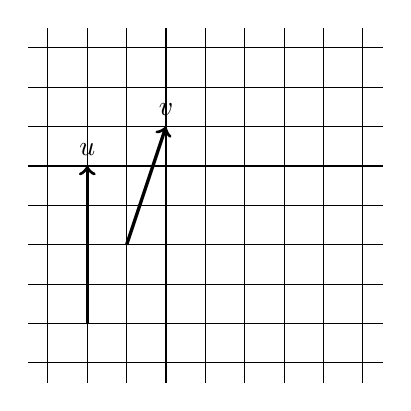
\begin{tikzpicture}
\draw (-0.25,-0.25) grid[step=0.5,color=gray!50] (4.25,4.25);
\draw[->,very thick] (0.5,0.5) -- ++(0,2) node[above] {$\vect{u}$}; 
\draw[->,very thick] (1,1.5) -- ++(0.5,1.5) node[above] {$\vect{v}$}; 
\end{tikzpicture}
\end{minipage}
\hfill
\begin{minipage}{0.25\textwidth}
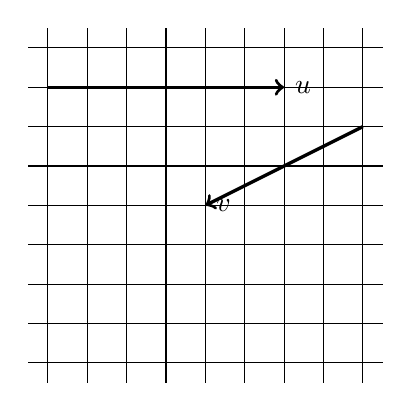
\begin{tikzpicture}
\draw (-0.25,-0.25) grid[step=0.5,color=gray!50] (4.25,4.25);
\draw[->,very thick] (0,3.5) -- ++(3,0) node[right] {$\vect{u}$};
\draw[->,very thick] (4,3) -- ++(-2,-1) node[right] {$\vect{v}$};
\end{tikzpicture}
\end{minipage}
\hfill
\begin{minipage}{0.25\textwidth}
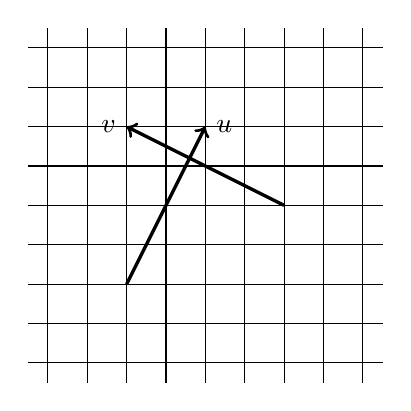
\begin{tikzpicture}
\draw (-0.25,-0.25) grid[step=0.5,color=gray!50] (4.25,4.25);
\draw[->,very thick] (1,1) -- ++(1,2) node[right] {$\vect{u}$};
\draw[->,very thick] (3,2) -- ++(-2,1) node[left] {$\vect{v}$};
\end{tikzpicture}
\end{minipage}
\hfill
\end{example}

\begin{tcolorbox}
\begin{definition}[Produit scalaire]
Soient $\vect{u}$ et $\vect{v}$ deux vecteurs. On appelle \textbf{produit scalaire} de $\vect{u}$ et de $\vect{v}$, noté $\vect{u} \cdot \vect{v}$, le nombre:
\begin{itemize}
\item $0$ si $\vect{u}$ est nul ou $\vect{v}$ est nul.
\item $\norm{\vect{u}} \times \norm{\vect{v}} \times \cos\left(\widehat{\vect{u},\vect{v}}\right)$ dans le cas contraire.
\end{itemize}
\end{definition}    
\end{tcolorbox}

\newpage

\section{Premières propriétés}
\subsection{Propriétés algébriques}
\begin{proposition}
Soient $\vect{u}$, $\vect{v}$ deux vecteurs du plan, ainsi que $k \in \R$.
\begin{enumerate}
\item On a $\vect{u} \cdot \vect{v} = \vect{v} \cdot \vect{u}$. (Le produit scalaire est \emph{symétrique})
\item On a $(k\vect{u}) \cdot \vect{v} = \vect{u} \cdot (k\vect{v}) = k \times (\vect{u} \cdot \vect{v})$.
\end{enumerate}
\end{proposition}
\begin{remark}
Attention à l'usage de $\cdot$ et de $\times$ : l'un concerne deux vecteurs, et l'autre deux nombres.
\end{remark}
\emptybox{2.5cm}
\begin{example}
Soit $\vect{u}$ et $\vect{v}$ deux vecteurs tels que $\norm{\vect{u}} = 2$, $\norm{\vect{v}} = 3$ et $\widehat{\vect{u};\vect{v}} = 30°$. Calculer les produits scalaires suivants.
\begin{enumerate}[label=\emph{\alph*)}]
\item $\vect{u} \cdot \vect{v} = $\answersline
\item $\vect{u} \cdot \vect{u} =$\answersline
\item $\vect{v} \cdot (2\vect{u}) =$\answersline
\item $(-4\vect{u}) \cdot (3\vect{v}) = $\answersline
\end{enumerate}
\end{example}
\subsection{Propriétés géométriques}
\begin{proposition}
Soient $\vect{u}$ et $\vect{v}$ deux vecteurs.
\begin{itemize}
\item Si $\vect{u}$ et $\vect{v}$ sont colinéaires de même sens, alors $\vect{u} \cdot \vect{v} = \norm{\vect{u}} \times \norm{\vect{v}}$; 
\item Si $\vect{u}$ et $\vect{v}$ sont colinéaires de sens opposés, alors $\vect{u} \cdot \vect{v} = - \norm{\vect{u}} \times \norm{\vect{v}}$; 
\end{itemize}    
\end{proposition}
\begin{tcolorbox}
\begin{definition}
Soient $\vect{u}$ et $\vect{v}$ deux vecteurs. Alors ces deux vecteurs sont dit \textbf{orthogonaux} si l'un des deux vecteurs est nul; ou si l'angle $\widehat{\vect{u};\vect{v}} = 90°$.
\end{definition}
\end{tcolorbox}
\begin{proposition}
Soient $\vect{u}$ et $\vect{v}$ deux vecteurs. Alors, $\vect{u}$ et $\vect{v}$ sont orthogonaux si et seulement si $\vect{u} \cdot \vect{v} = 0$.    
\end{proposition}
\begin{remark}
\begin{itemize}
\item Cette proposition est facile à démontrer avec notre définition, mais sera surtout utile avec les définitions suivantes.
\item Le vecteur nul est donc orthogonal à tous les vecteurs.
\end{itemize}
\end{remark}
\subsection{Définition avec le projeté orthogonal}
\begin{tcolorbox}
    
\begin{definition}[Rappel]
Soit $M$ un point du plan et $(d)$ une droite. Le \textbf{projeté orthogonal} de $M$ par rapport à la droite $(d)$ est l'unique point $M'$ appartenant à la droite $(d)$ et tel que les droite $(MM')$ et $(d)$ sont perpendiculaires.
\end{definition}
\end{tcolorbox}
\begin{proposition}
Soient $\vect{u}$ et $\vect{v}$ deux vecteurs non nuls. On pose $A$, $B$ et $C$ tels que $\vect{u} = \vect{AB}$ et $\vect{v} = \vect{AC}$. De plus, on pose $H$ le projeté orthogonal de $C$ par rapport à la droite $AB$. Alors,
\begin{equation*}
\vect{u} \cdot \vect{v} = 
\begin{cases}
AB \times AH & \text{ si $\vect{AB}$ et $\vect{AH}$ sont de même sens;}\\
- AB \times AH& \text{ si $\vect{AB}$ et $\vect{AH}$ sont de sens opposés.}
\end{cases}
\end{equation*}
\end{proposition}
\emptybox{3cm}

\newpage
\section{Produit scalaire en géométrie repérée}
On munit le plan d'un repère orthonormée $(O,I,J)$. Les coordonnées d'un vecteur $\vect{u}$ d'abscisse $x$ et d'ordonnée $y$ sont notées
\begin{equation*}
\vect{u}\vcoord{x}{y}
\end{equation*}
\subsection{Bilinéarité du produit scalaire}
\begin{proposition}
Soient trois vecteurs $\vect{u}$, $\vect{v}$ et $\vect{w}$. Alors,
\begin{equation*}
\vect{u} \cdot (\vect{v} + \vect{w}) = \vect{u} \cdot \vect{v} + \vect{u} \cdot \vect{w}
\end{equation*}
\end{proposition}
\begin{remark}
Ce résultat correspond donc à la distributivité du produit scalaire sur l'addition de vecteurs.
\end{remark}
\begin{example}
Soient trois vecteurs $\vect{u}$, $\vect{v}$ et $\vect{w}$ de norme $1$ tels que $\vect{u} \cdot \vect{v}$ = $\dfrac{\sqrt{3}}{2}$  et $\vect{u} \cdot \vect{w}$ = $\dfrac{1}{\sqrt{2}}$. Que vaut $\vect{u} \cdot (\vect{v} + \vect{w})$ ?

\answersline
\end{example}
\subsection{Définition en géométrie repérée}
\begin{proposition}
Soient deux vecteurs $\vect{u}\vcoord{x_u}{y_u}$ et $\vect{v}\vcoord{x_v}{y_v}$. Alors, le produit scalaire $\vect{u} \cdot \vect{v}$ est égal à
\begin{equation*}
x_u \times x_v + y_u \times y_v    
\end{equation*}
\end{proposition}
\begin{example}
Calculer le produit scalaire des vecteurs $\vect{u}$ et $\vect{v}$ suivants
\begin{enumerate}[label=\emph{\alph*)}]
\begin{minipage}{0.45\textwidth}
\item $\vect{u}\vcoord{2}{3}$ et $\vect{v}\vcoord{3}{4}$ : $\vect{u} \cdot \vect{v} =$ \answersline
\item $\vect{u}\vcoord{1}{-7}$ et $\vect{v}\vcoord{3}{4}$ : $\vect{u} \cdot \vect{v} =$ \answersline
\end{minipage}
\hfill    
\begin{minipage}{0.45\textwidth}
\item $\vect{u}\vcoord{-4}{5}$ et $\vect{v}\vcoord{5}{4}$ : $\vect{u} \cdot \vect{v} =$ \answersline
\item $\vect{u}\vcoord{6}{9}$ et $\vect{v}\vcoord{9}{12}$ : $\vect{u} \cdot \vect{v} =$ \answersline
\end{minipage}
\end{enumerate}
\end{example}
\subsection{Produit scalaire et norme}
\begin{proposition}
Soit $\vect{u}\vcoord{x}{y}$ un vecteur. Alors,
\begin{equation*}
\norm{\vect{u}}^2 = \vect{u} \cdot \vect{u} = x^2 + y^2
\end{equation*}
\end{proposition}
\begin{proposition}[Identités remarquables]
Soient $\vect{u}$ et $\vect{v}$ deux vecteurs. Alors
\begin{equation*}
\begin{cases}
\norm{\vect{u} + \vect{v}}^2 &= \norm{\vect{u}}^2 + 2(\vect{u} \cdot \vect{v})+ \norm{\vect{v}}^2\\
\norm{\vect{u} - \vect{v}}^2 &= \norm{\vect{u}}^2 - 2(\vect{u} \cdot \vect{v})+ \norm{\vect{v}}^2\\
(\vect{u} - \vect{v}) \cdot (\vect{u} + \vect{v}) &= \norm{\vect{u}}^2 - \norm{\vect{v}}^2
\end{cases}
\end{equation*}
\end{proposition}
\begin{tcolorbox}
\begin{proposition}
Soient $\vect{u}$ et $\vect{v}$ deux vecteurs. Alors,
\begin{equation*}
\vect{u} \cdot \vect{v} = \dfrac{1}{2}(\norm{\vect{u} + \vect{v}}^2 - \norm{\vect{u}}^2 - \norm{\vect{v}}^2) = \dfrac{1}{2}(\norm{\vect{u}}^2 + \norm{\vect{v}}^2 - \norm{\vect{u - v}}^2)
\end{equation*}
\end{proposition}
\end{tcolorbox}
\end{document}